% !TEX root = ../Dokumentation.tex
\subsection{Objekterkennung}
Die Objekterkennung hat das Ziel die richtigen Objekte zu erkennen und das genaue Positionieren des Fahrzeuges zu ermöglichen. Dabei wird die Containererkennung in zwei Teilaufgaben aufgeteilt: Die \glqq{Objekterkennung grob}\grqq{} ist für die Erkennung der richtigen Objekte mittels Farb- und Formerkennung zuständig. Die \glqq{Objekterkennung präzise}\grqq{} ist für das Positionieren des Fahrzeuges notwendig. Diese zwei Teilaufgaben werden separat angeschaut.
%
\subsubsection{Objekterkennung grob}
Die Aufgabe der \glqq{Objekterkennung grob}\grqq ist es, die aufzuladenden Container, kreuzenden Fahrzeuge und das Entleerungsbecken zu erkennen. Sobald ein solches Objekt erkannt wird, wird der zentrale Controller darüber informiert, damit die Informationen an die \glqq{Objekterkennung}\grqq{} präzise weitergegeben werden können.
\\[0.2cm]
\underline{\textbf{Container}}
\\[0.2cm]
\textbf{Funktionsbeschrieb}\\[0.2cm]
Bei der Container- und Entleerungsbeckenerkennung werden grüne und blaue Container erkannt. Wird eines dieser Objekte erkannt, wird der Controller darüber informiert, damit sich das Fahrzeug auf das Aufladen vorbereiten kann. Das Entleerungsbecken wird nicht mehr, wie in der Konzeptphase geplant, über die Objekterkennung erkannt. Da das Entleerungsbecken weiss ist, würde es bei der Farberkennung zu viele Störobjekte haben. Neu ist die Fahrbahnerkennung dafür verantwortlich.
\\[0.2cm]
Sobald die ersten Bilder mit der Kamera aufgenommen wurden, werden diese laufend aus dem Bilderpool abgefragt und untersucht. Dabei läuft die Erkennung von grünen und blauen Containern parallel ab.
\begin{figure}[H]%Position festigen
\centering
\includegraphics[width=0.6\textwidth]{03_Loesungskonzept/pictures/objekterkennung_containers.png}
\caption{Aktivitätendiagramm Obkjekterkennung: Container und Entleerungsbecken}
\label{fig:activityContainer}
\end{figure}
\newpage
Die Erkennung läuft dabei immer gleich ab. Als erstes wird das Bild mit OpenCV nach der entsprechenden Farbe gefiltert. Sprich: Es wird nur nach Grün- und Blautönen gesucht. Anschliessend werden mit Hilfe einer Konturerkennung störende und falsche Objekte entfernt. Mit der Höhe dieser Objekte kann dann ausgerechnet werden, wie weit das Objekt  noch entfernt ist. Diese Distanzberechnung liefert nur ein ungefähres Ergebnis. Ist das Objekt zu weit entfernt, wird der zentrale Controller nicht informiert. Ansonsten wird eine Meldung an den Controller gesendet, welche die Distanz enthält. Die folgende Darstellung soll die einzelnen Schritte verdeutlichen.
\\[0.2cm]


\underline{\textbf{Rechtsvortritt}}
Damit Kollisionen mit anderen Fahrzeugen vermieden werden können, wurde ein Ultraschallsensor eingebaut. Dieser misst über kurze Ultraschallpulse die Distanz zum nächsten Objekt. Die Ansteuerung und Auswertung wurde auf dem Mikrocontrollerboard realisiert. Die Grundlage der Implementierung basiert auf diesem Tutorial: https://mcuoneclipse.com/2013/01/01/tutorial-ultrasonic-ranging-with-the-freedom-board/. Jedoch wurde dieser Code noch effizienter gestaltet.\\[0.2cm]
\textbf{Vergleich Konzept und Umsetzung}\\[0.2cm]
Die Ansteuerung des Ultraschallsensor konnte bereits im Pren1 als Funktionsmuster erfolgreich getestet werden. Daher musste im Pren2 nichts am bestehenden Konzept geändert werden.


\subsubsection{Objekterkennung präzise}
\underline{\textbf{Containererkennung}}\\[0.2cm]
Das präzise Stoppen beim Container wird vom Freedomboard gesteuert. Der Aufladevorgang 
\textbf{Vergleich Konzept und Umsetzung}\\[0.2cm]
Das Konzept mit dem präzisen anhalten über den Infrarotsensor hat sich im Pren2 nicht geändert.
\begin{figure} [H]
	\centering
	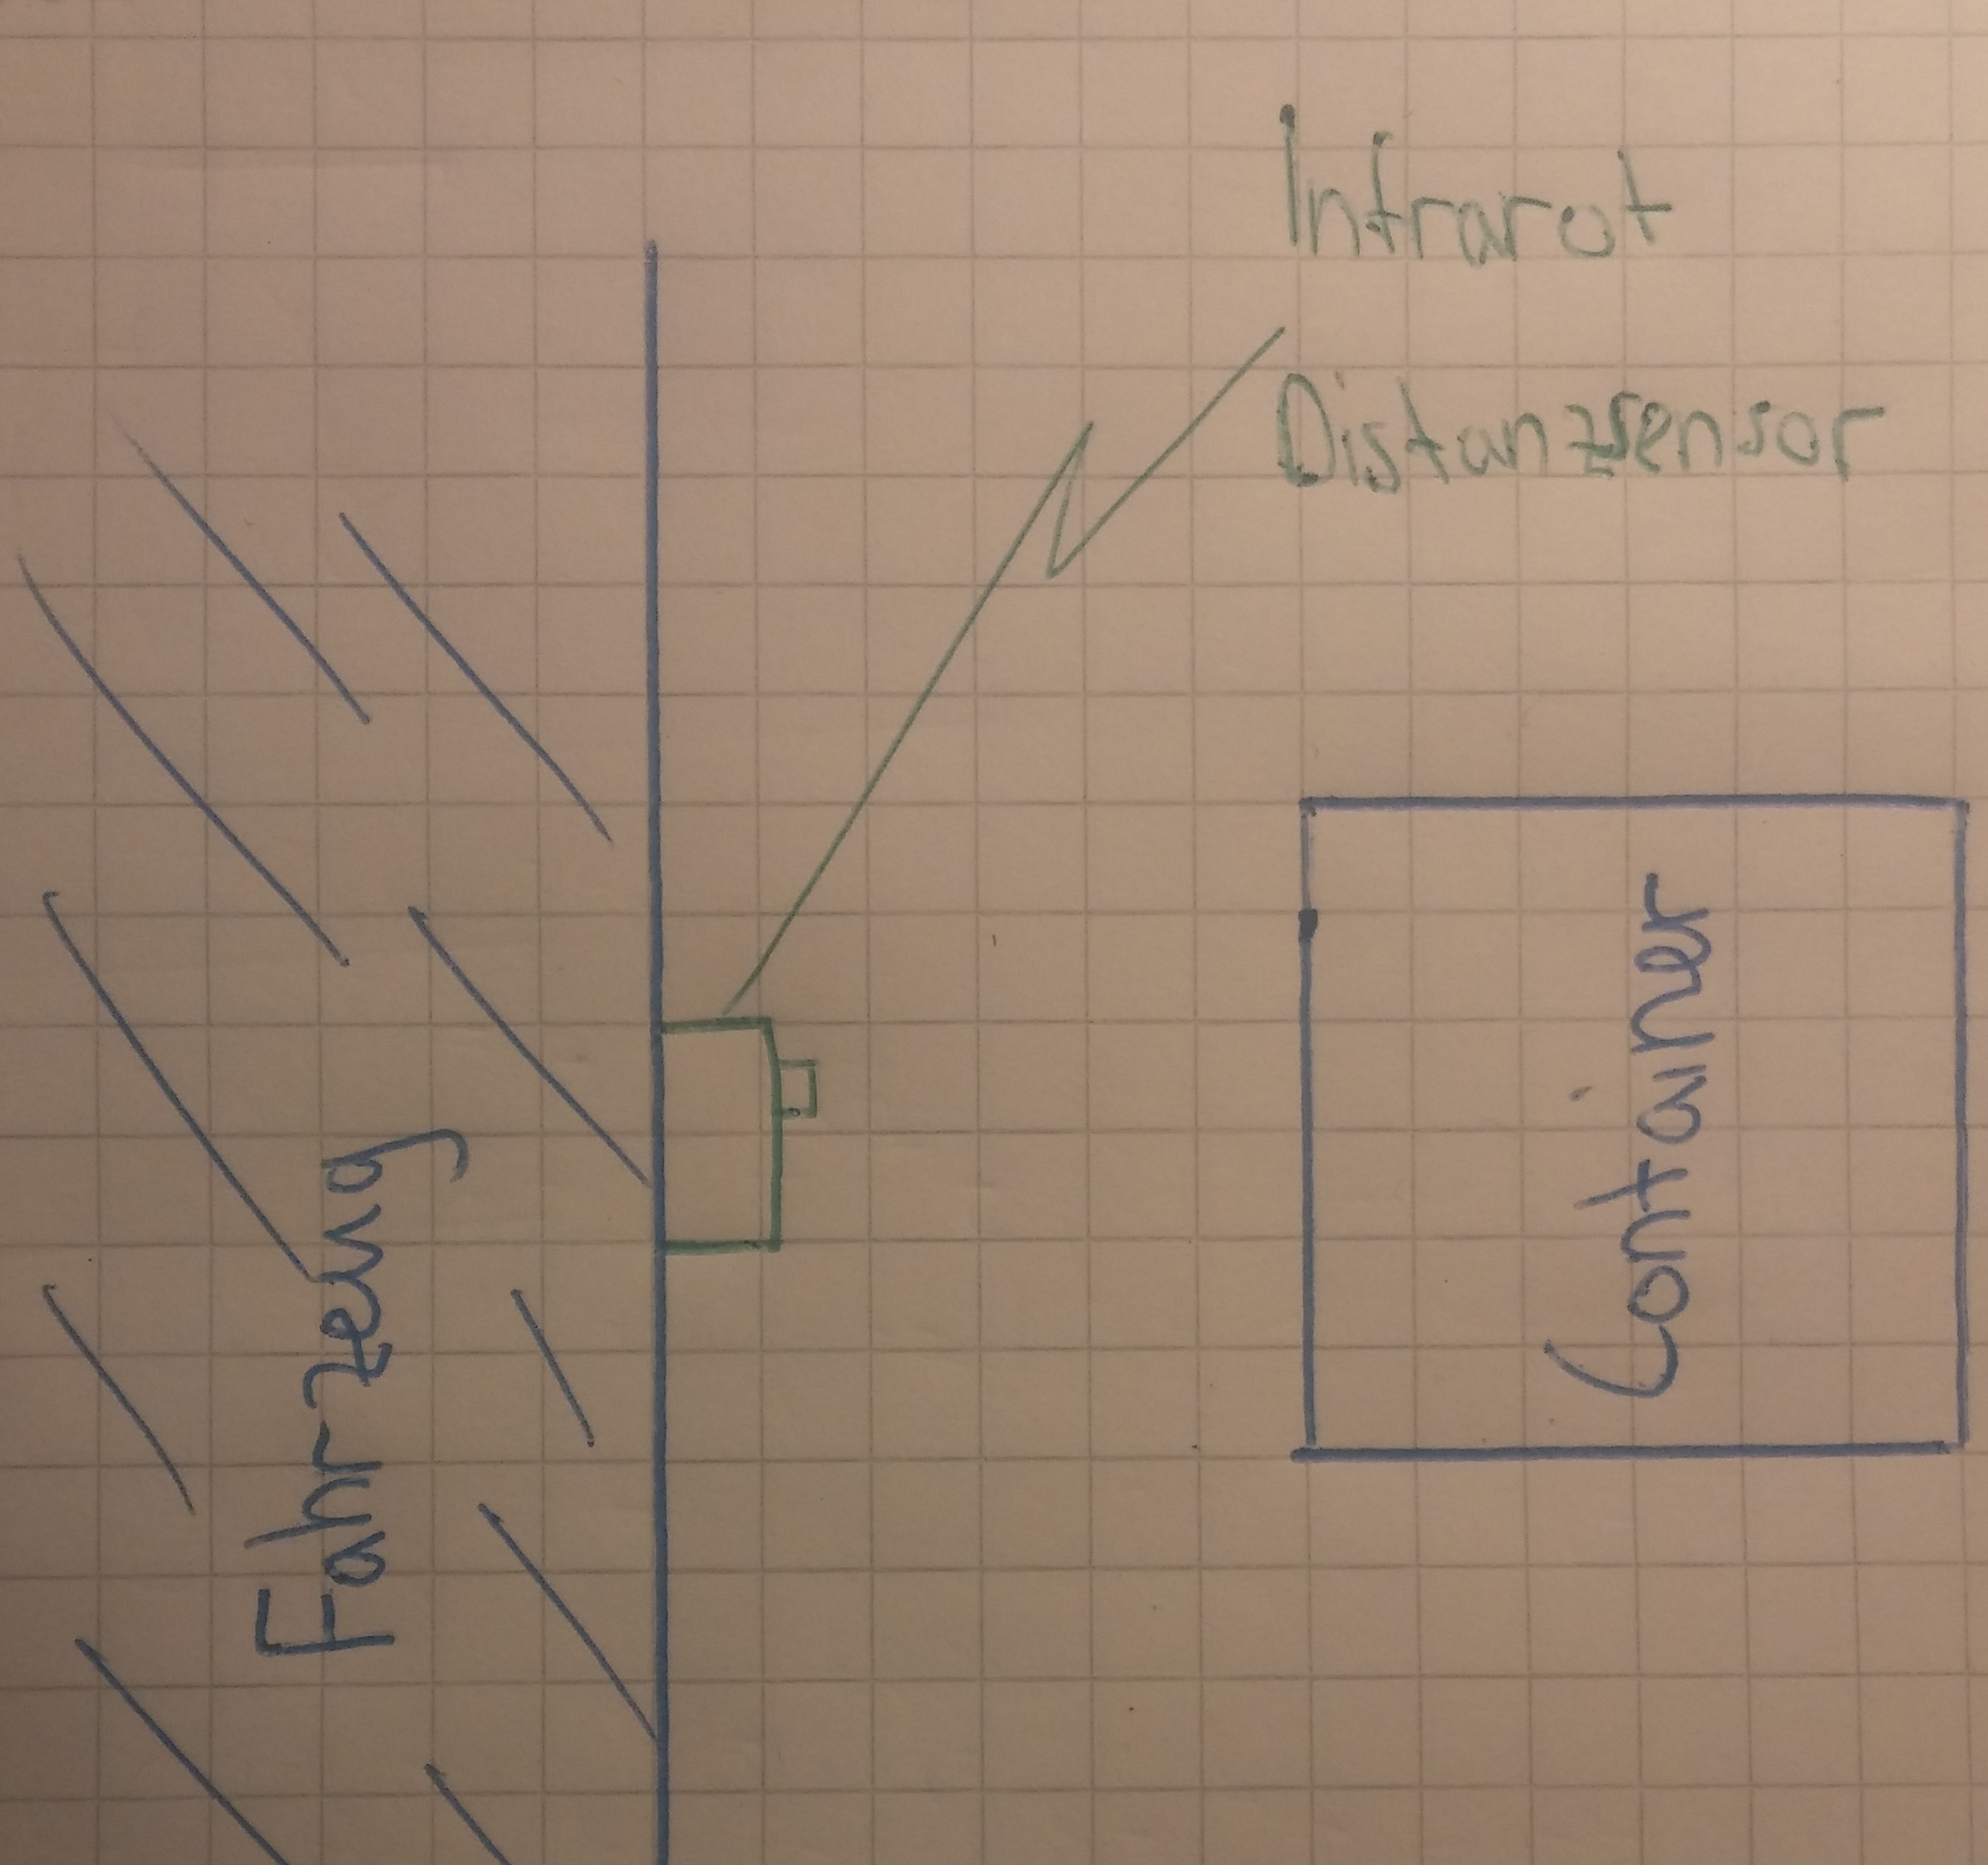
\includegraphics[width=0.35\textwidth]{03_Loesungskonzept/pictures/InfrarotContainererkennung.png}
	\caption{Beispielhafte Containererkennung mit einem Infrarotsensor}
\end{figure}
\textbf{Begründung}\\[0.2cm]
Die Positionierung mit einem Infrarotsensor ist die ideale Lösung. Sie ist einfach zu realisieren im Vergleich zu einer Kamera oder einem Farbesensor und präziserer als ein Ultraschallsensor.\\[0.2cm]
\textbf{Testergebnisse}\\[0.2cm]
Für die Ermittlung des besten Sensors wurde ein Ultraschall und Infrarotsensor als Funktionsmuster getestet. Der relativ grosse \glqq{Empfangswinkel}\grqq, welcher der Ultraschallsensor aufweist, ist in dieser Anwendung nicht gewollt. Der Infrarotsensor ist diesbezüglich besser. Dieser ist zwar lichtempfindlich, jedoch sollte dieses Problem gelöst werden können.\\[0.2cm]
%
\underline{\textbf{Rechtsvortritt}} \\[0.2cm]
\textbf{Funktionsbeschrieb}\\[0.2cm]
Die \glqq{Rechtsvortritterkennung detailliert}\grqq{} hat die Aufgabe das Fahrzeug vor einer Kollision mit einem zweiten Fahrzeug zu bewahren. Wenn rechts oder vor dem Fahrzeug etwas im Weg ist, soll das Fahrzeug anhalten.\\[0.2cm]
\textbf{Komponentenbeschrieb}\\[0.2cm]
\begin{figure} [H]
	\centering
	\includegraphics[width=0.23\textwidth]{03_Loesungskonzept/pictures/ultraschallsensor.png}
	\caption{Getesteter Ultraschallsensor (Quelle: www.generationrobots.com)}
	%http://www.generationrobots.com/2653-large_default/ultraschallsensor-hc-sr04.jpg
\end{figure}
Diese Aufgabe wird mit einem Ultraschallsensor gelöst. \\[0.2cm]
\textbf{Begründung}\\[0.2cm]
Ein Ultraschallsensor ist für unter fünf Franken zu haben und erfüllt mit seinem grossen Abstrahlwinkel und seiner Reichweite die geforderten Bedingungen. Zudem ist die Anbindung an das Freedomboard gut möglich.\\[0.2cm]
\textbf{Testergebnisse}\\[0.2cm]
Der Ultraschallsensor wurde bereits erfolgreich an das Freedomboard angeschlossen und  ausgewertet. Die Anbindung wurde mit Hilfe einer Anleitung von mcuoneclipse.com realisiert. Die Distanzauswertung funktionierte bei dem Test relativ genau ($\approx \pm $ 1cm).\\[0.2cm]
%
\underline{\textbf{Entleerungbecken Erkennung}} \\[0.2cm]
\textbf{Funktionsbeschrieb}\\[0.2cm]
Damit das Schüttgut im Entleerungsbecken entleert werden kann, muss das Entleerungsbecken richtig detektiert werden können. \\[0.2cm]
\textbf{Komponentenbeschrieb}\\[0.2cm]
Die Container und Fahrbahnerkennung benötigen bereits Sensoren. Dies wären der Flexsensor und der Infrarotsensor. Für die Detektion des Entleerungsbehälters ist kein weiterer Sensor mehr nötig. Die Detektion ist mit beiden Sensoren möglich. Bei Tests mit den beiden Sensoren wird sich zeigen, welcher dieser beiden besser geeignet ist.\\[0.2cm]
\textbf{Begründung}\\[0.2cm]
Die Einsparung von Sensoren entlastet das Budget und spart zusätzlichen Implementierungsaufwand.\\[0.2cm]